\documentclass{standalone}
\usepackage{tikz} % tikz
\usepackage{standalone} % tikz figures are often in standalone
\usepackage{amsfonts} % mathbb etc
\usepackage{amsmath} % crucial package
\usepackage{amsthm} % ams-style theorems
\usepackage{bm} % bold math symbols
\usepackage{xcolor} % more colors
\usepackage[T1]{fontenc} % modern encoding, better than OT1, the default

\newtheorem{definition-fr}{Définition}
\newtheorem{example-fr}{Exemple}
\newtheorem{theorem-fr}{Théorème}
\newtheorem{proposition-fr}{Proposition}
\newtheorem{lemma-fr}{Lemme}
\newtheorem{remark-fr}{Remarque}
\newtheorem{definition}{Definition}
\newtheorem{lemma}{Lemma}
\newtheorem{proposition}{Proposition}
\newtheorem{remark}{Remark}

\usetikzlibrary{decorations.pathmorphing} % for snake, zigzag...
\usetikzlibrary{positioning} % for the "below of=1cm" type of options
\usetikzlibrary{intersections} % e.g. for pyramid
\usetikzlibrary{calc} % for computing node coordinates from others
\usetikzlibrary{overlay-beamer-styles} % when \pause glitches in tikz beamer
\usetikzlibrary{arrows} % arrows
\usetikzlibrary{external} % only compile the figure the first time
\tikzexternalize[only named=true, prefix=tikz-cache/]
\immediate\write18{mkdir -p latex-build/tikz-cache}

% used to pass "scale=XX" as includetikz option
\pgfkeys{
  /tikzoptions/.is family, % Namespace
  /tikzoptions/.cd, % Namespace
  scale/.store in=\scale, % Store the value of 'scale'
}

% usage: \includetikz[scale=XX]{fig}, fetches from my local database
\newcommand{\includetikz}[2][scale=1]{
  \bgroup
  \pgfkeys{/tikzoptions,#1} % currently only accepts 'scale' (april 9 2025)
  \tikzsetnextfilename{#2}
  \include{tex-macros/tikz-figures/#2}% Include the standalone TikZ file
  \egroup
}

% usage: \inputtikz[scale=XX]{fig}, fetches from my local database
\newcommand{\inputtikz}[2][scale=1]{
  \bgroup
  \pgfkeys{/tikzoptions,#1} % currently only accepts 'scale' (april 9 2025)
  \tikzsetnextfilename{#2}
  \input{tex-macros/tikz-figures/#2}% Include the standalone TikZ file
  \egroup
}


\newcommand{\bigOt}{\widetilde{\mathcal{O}}}
\newcommand{\bigO}{\mathcal{O}}

\definecolor{mypurp}{HTML}{8f0c97}
\definecolor{myred}{HTML}{9f103b}
\definecolor{myor}{HTML}{ae3011}
\definecolor{mydarkor1}{HTML}{96240f}
\definecolor{mydarkor2}{HTML}{7f180c}
\definecolor{mylb1}{HTML}{00557e}
\definecolor{mylb2}{HTML}{013157}
\definecolor{mybl1}{HTML}{0d08a9}
\definecolor{mybl2}{HTML}{04037f}
\definecolor{mygr1}{HTML}{097e3e}
\definecolor{mygr2}{HTML}{025520}
\definecolor{myyellow}{HTML}{FFD700}



\makeatletter
\@ifundefined{scale}{
  \def\scale{1}
}
\makeatother


\begin{document}
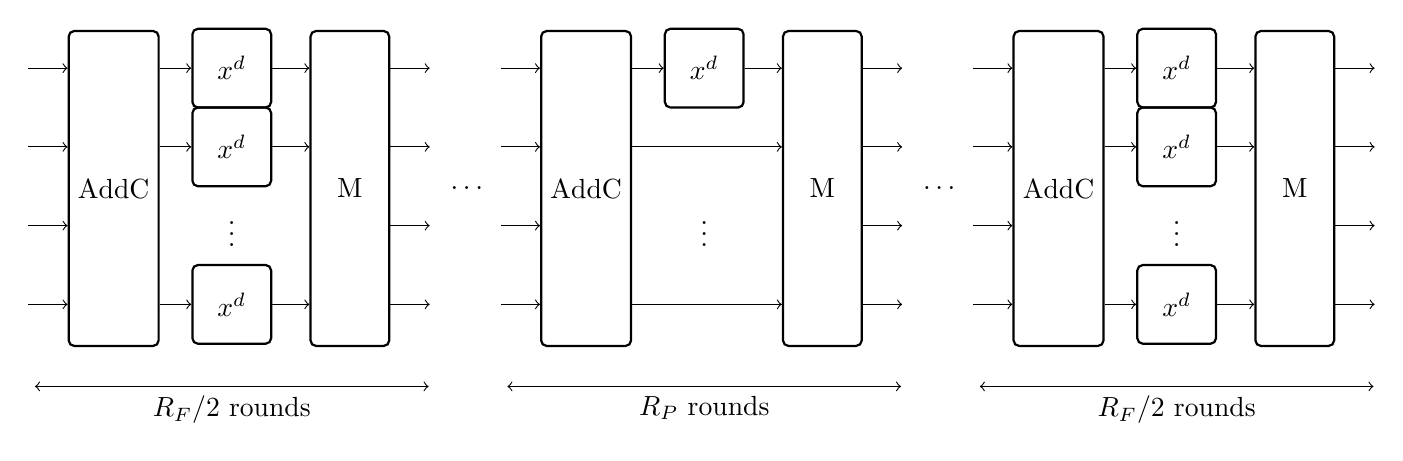
\begin{tikzpicture}[
	scale = \scale,
	transform shape,
	sbox/.style={rounded corners=2pt, rectangle, draw, thick, minimum size = 1cm, anchor=south},	
	outer/.style={rounded corners=2pt, rectangle, draw, thick, minimum height = 4cm, minimum width = 1cm, anchor=south},
	]
	
	\begin{scope}[xshift=-6cm,name prefix=RF1/]
		\node[outer] (AddC) at (0.5,0) {AddC};
		\node[sbox] (s1) at ([xshift=1.5cm, yshift=-1cm] AddC.north) {$x^d$};
		\node[sbox] (s2) at ([xshift=1.5cm, yshift=-2cm] AddC.north) {$x^d$};
		\node[sbox, draw=none] (s3) at ([xshift=1.5cm, yshift=-3cm] AddC.north) {$\vdots$};
		\node[sbox] (s4) at ([xshift=1.5cm, yshift=-4cm] AddC.north) {$x^d$};
		\node[outer, anchor=center] (MDS) at ([xshift=3cm,yshift = 0] AddC) {M};

		\draw[->] (AddC.east|-s1.west) -- (s1.west);
		\draw[->] (AddC.east|-s2.west) -- (s2.west);
		\draw[->] (AddC.east |-s4.west) -- (s4.west);

		\draw[<-]  (AddC.west|-s1.west) -- ++(-0.5,0);
		\draw[<-]  (AddC.west|-s2.west) -- ++(-0.5,0);
		\draw[<-]  (AddC.west|-s3.west) -- ++(-0.5,0);
		\draw[<-]  (AddC.west|-s4.west) -- ++(-0.5,0);

		\draw[->] (s1.east) -- (MDS.west|-s1.west); 
		\draw[->] (s2.east) -- (MDS.west|-s2.east);
		\draw[->] (s4.east) -- (MDS.west|-s4.east);

		\draw[->]  (MDS.east|-s1.west) -- ++(+0.5,0);
		\draw[->]  (MDS.east|-s2.west) -- ++(+0.5,0);
		\draw[->]  (MDS.east|-s3.west) -- ++(+0.5,0);
		\draw[->]  (MDS.east|-s4.west) -- ++(+0.5,0);

		\draw[<->]
        ($(AddC.south) + (-1cm, -0.5cm)$) -- 
        ($(MDS.south) + (1cm, -0.5cm)$) node[midway, below] {$R_F/2$ rounds};

	\end{scope}

	\node[sbox,draw=none,right=1cm of RF1/MDS.center] {\dots};

	\begin{scope}[xshift=0cm,name prefix=RF2/]
		\node[outer] (AddC) at (0.5,0) {AddC};
		\node[sbox] (s1) at ([xshift=1.5cm, yshift=-1cm] AddC.north) {$x^d$};
		\node[sbox, draw=none] (s2) at ([xshift=1.5cm, yshift=-2cm] AddC.north) {};
		\node[sbox, draw=none] (s3) at ([xshift=1.5cm, yshift=-3cm] AddC.north) {$\vdots$};
		\node[sbox, draw=none] (s4) at ([xshift=1.5cm, yshift=-4cm] AddC.north) {};
		\node[outer, anchor=center] (MDS) at ([xshift=3cm,yshift = 0] AddC) {M};

		\draw[->] (AddC.east|-s1.west) -- (s1.west);
	
		\draw[<-]  (AddC.west|-s1.west) -- ++(-0.5,0);
		\draw[<-]  (AddC.west|-s2.west) -- ++(-0.5,0);
		\draw[<-]  (AddC.west|-s3.west) -- ++(-0.5,0);
		\draw[<-]  (AddC.west|-s4.west) -- ++(-0.5,0);

		\draw[->] (s1.east) -- (MDS.west|-s1.west); 
		\draw[->] (AddC.east|-s2.east) -- (MDS.west|-s2.east);
		\draw[->] (AddC.east|-s4.east) -- (MDS.west|-s4.east);

		\draw[->]  (MDS.east|-s1.west) -- ++(+0.5,0);
		\draw[->]  (MDS.east|-s2.west) -- ++(+0.5,0);
		\draw[->]  (MDS.east|-s3.west) -- ++(+0.5,0);
		\draw[->]  (MDS.east|-s4.west) -- ++(+0.5,0);

		\draw[<->]
        ($(AddC.south) + (-1cm, -0.5cm)$) -- 
        ($(MDS.south) + (1cm, -0.5cm)$) node[midway, below] {$R_P$ rounds};

	\end{scope}

	\node[sbox,draw=none,right=1cm of RF2/MDS.center] {\dots};

	\begin{scope}[xshift=6cm,name prefix=RF3/]
		\node[outer] (AddC) at (0.5,0) {AddC};
		\node[sbox] (s1) at ([xshift=1.5cm, yshift=-1cm] AddC.north) {$x^d$};
		\node[sbox] (s2) at ([xshift=1.5cm, yshift=-2cm] AddC.north) {$x^d$};
		\node[sbox, draw=none] (s3) at ([xshift=1.5cm, yshift=-3cm] AddC.north) {$\vdots$};
		\node[sbox] (s4) at ([xshift=1.5cm, yshift=-4cm] AddC.north) {$x^d$};
		\node[outer, anchor=center] (MDS) at ([xshift=3cm,yshift = 0] AddC) {M};

		\draw[->] (AddC.east|-s1.west) -- (s1.west);
		\draw[->] (AddC.east|-s2.west) -- (s2.west);
		\draw[->] (AddC.east |-s4.west) -- (s4.west);

		\draw[<-]  (AddC.west|-s1.west) -- ++(-0.5,0);
		\draw[<-]  (AddC.west|-s2.west) -- ++(-0.5,0);
		\draw[<-]  (AddC.west|-s3.west) -- ++(-0.5,0);
		\draw[<-]  (AddC.west|-s4.west) -- ++(-0.5,0);

		\draw[->] (s1.east) -- (MDS.west|-s1.west); 
		\draw[->] (s2.east) -- (MDS.west|-s2.east);
		\draw[->] (s4.east) -- (MDS.west|-s4.east);

		\draw[->]  (MDS.east|-s1.west) -- ++(+0.5,0);
		\draw[->]  (MDS.east|-s2.west) -- ++(+0.5,0);
		\draw[->]  (MDS.east|-s3.west) -- ++(+0.5,0);
		\draw[->]  (MDS.east|-s4.west) -- ++(+0.5,0);


		\draw[<->]
        ($(AddC.south) + (-1cm, -0.5cm)$) -- 
        ($(MDS.south) + (1cm, -0.5cm)$) node[midway, below] {$R_F/2$ rounds};

	\end{scope}

\end{tikzpicture}
\end{document}
